\documentclass[11pt,a4paper]{article}
\usepackage[T1]{fontenc}
\usepackage[utf8]{inputenc}
\usepackage{lmodern}
\usepackage{textcomp}
\usepackage[left=1.8cm,right=1.8cm,top=3.0cm,bottom=2.2cm,headheight=36pt,headsep=12pt]{geometry}
\usepackage{multicol}
\usepackage{xcolor}
\usepackage{fancyhdr}\usepackage{tikz}
\usepackage{graphicx}
\usepackage{array}
\usepackage{amsmath,amssymb}
\usepackage{setspace}
\usepackage{longtable}
\graphicspath{{../}}
\definecolor{ygreen}{RGB}{46,139,87}\definecolor{dgreen}{RGB}{28,90,56}
\renewcommand{\normalsize}{\fontsize{10.9}{13.4}\selectfont}
\renewcommand{\familydefault}{\rmdefault}
\setlength{\parindent}{0pt}
\setlength{\columnsep}{0.8cm}
\setlength{\columnseprule}{0.4pt}
\setlength{\multicolsep}{3pt plus 1pt minus 1pt}
\renewcommand{\textsubscript}[1]{\ensuremath{_{\text{\fontsize{8}{8}\selectfont #1}}}}
\renewcommand{\textsuperscript}[1]{\ensuremath{^{\text{\fontsize{8}{8}\selectfont #1}}}}
\newcommand{\qn}[1]{\textbf{\fontsize{11.5}{13}\selectfont #1}}
\newcommand{\qsep}{\par\vspace{13pt}}
\newcommand{\fwrule}{\par\vspace{5pt}\noindent\rule{\linewidth}{1.4pt}\par\vspace{7pt}}
\newsavebox{\fitb}
\newcommand{\fitbox}[1]{\sbox{\fitb}{#1}\ifdim\wd\fitb>\linewidth\resizebox{\linewidth}{!}{\usebox{\fitb}}\else\usebox{\fitb}\fi}
\newcommand{\diqqat}[1]{\par\smallskip\noindent\textbf{Diqqat!} #1\par\medskip}
\newcommand{\javob}{\par\nopagebreak[4]\smallskip\noindent\textbf{Javob:} \rule[-2pt]{7.5cm}{0.4pt}\par\smallskip\noindent\textbf{Diqqat!} Javobingizni javoblar varaqasiga ko`chirib yozing.\par\medskip}
\pagestyle{fancy}
\fancyhf{}
\renewcommand{\headrulewidth}{1.6pt}\renewcommand{\headrule}{{\color{ygreen}\hrule height 1.6pt width\headwidth}}
\newcommand{\hdrlogo}{
\begin{tikzpicture}[baseline=0pt]\fill[ygreen,rounded corners=3pt] (0,0) rectangle (0.95,0.95);\node[white,font=\fontsize{24}{26}\bfseries\selectfont] at (0.475,0.47){K};\node[anchor=west,font=\fontsize{16}{18}\bfseries\selectfont,text=dgreen] at (1.15,0.66){KIMYO};\node[anchor=west,font=\footnotesize\scshape,text=gray] at (1.15,0.2){Milliy sertifikat\ \ 2026};\end{tikzpicture}}
\newcommand{\hdrpill}[1]{\begin{tikzpicture}[baseline=0pt]\node[fill=ygreen,text=white,rounded corners=8pt,inner xsep=10pt,inner ysep=5pt,font=\fontsize{13}{15}\bfseries\selectfont] at (0,0.475){#1};\end{tikzpicture}}
\fancyhead[L]{\hdrlogo}
\fancyhead[R]{\hdrpill{15-variant}}

\fancyfoot[C]{\thepage}
\fancypagestyle{first}{\fancyhf{}\renewcommand{\headrulewidth}{1.6pt}\renewcommand{\headrule}{{\color{ygreen}\hrule height 1.6pt width\headwidth}}\fancyhead[L]{\hdrlogo}\fancyhead[R]{\hdrpill{15-variant}}\fancyfoot[C]{\thepage}}
\begin{document}
\normalsize
\thispagestyle{first}
\noindent\textit{Davriy jadvaldan foydalanish mumkin.}
\par\smallskip
\begin{multicols}{2}
\noindent\qn{1.} 29-tartib raqamli element atomida bosh kvant soni n = 2, orbital kvant soni l = 1 bo`lgan elektronlar soni nechta?

\noindent A)~\textsl{7} \hfill B)~\textsl{5} \hfill C)~\textsl{6} \hfill D)~\textsl{8}\par
\qsep
\noindent\qn{2.} Doimiy tok kuchida Ag tuzining eritmasi elektroliz qilinganda katodda ajralgan metall massasining vaqtga bog`liqligi grafikda berilgan (M(Ag) = 108 g/mol, valentlik 1).
\begin{center}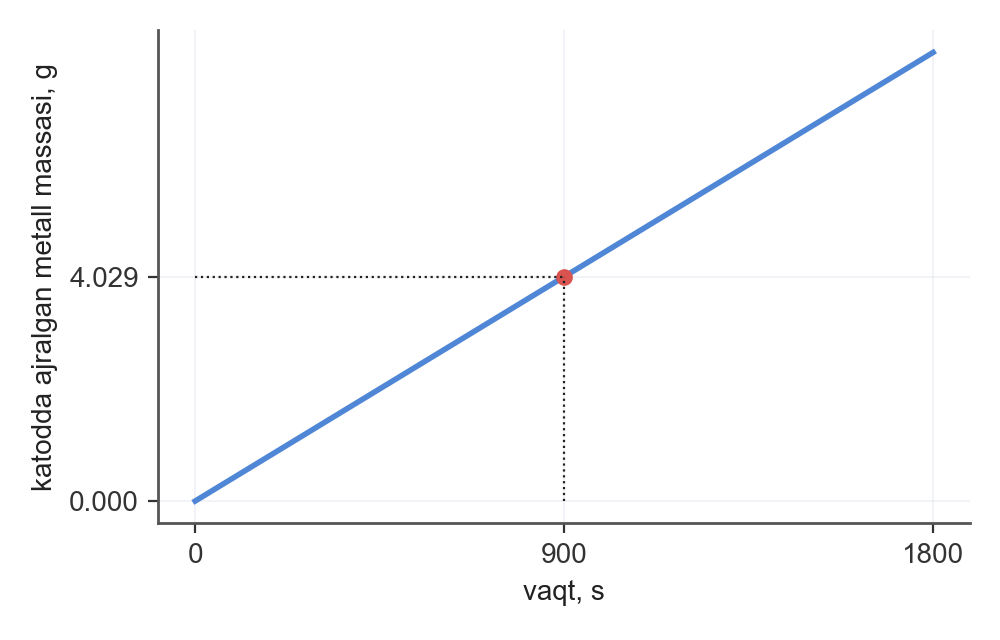
\includegraphics[width=0.86\linewidth]{rasmlar/gen/fa_v15_0.png}\end{center}
Grafikdagi nuqtaga mos kelgan jarayonda elektrodlardan o`tgan zaryad \textbf{miqdorini (C) hisoblang.}

\noindent A)~\textsl{3600} \hfill B)~\textsl{7200} \hfill C)~\textsl{1800} \hfill D)~\textsl{388800}\par
\qsep
\noindent\qn{3.} 0,1 M Ca(OH)\textsubscript{2} eritmasining normal \textbf{konsentratsiyasini (n) aniqlang.}

\noindent A)~\textsl{0,1} \hfill B)~\textsl{0,4} \hfill C)~\textsl{0,05} \hfill D)~\textsl{0,2}\par
\qsep
\noindent\qn{4.} Jadvalda bog`lar hosil qiluvchi atomlarning elektrmanfiyliklari berilgan:
\begin{center}
\renewcommand{\arraystretch}{1.15}
\fitbox{\begin{tabular}{|c|c|c|}\hline
\textbf{Bog`} & \textbf{EM (1-atom)} & \textbf{EM (2-atom)} \\ \hline
N--H & 3 & 2,1 \\ \hline
Na--Cl & 0,9 & 3 \\ \hline
H--O & 2,1 & 3,5 \\ \hline
H--Cl & 2,1 & 3 \\ \hline
\end{tabular}}
\end{center}
Qaysi bog` eng qutbli (eng ko`p ionli xarakterga ega)?

\noindent A)~\textsl{N--H} \hfill B)~\textsl{Na--Cl} \hfill C)~\textsl{H--O} \hfill D)~\textsl{H--Cl}\par
\qsep
\noindent\qn{5.} 0,2 M H\textsubscript{2}SO\textsubscript{4} eritmasining normal \textbf{konsentratsiyasini (n) aniqlang.}

\noindent A)~\textsl{0,4} \hfill B)~\textsl{0,2} \hfill C)~\textsl{0,8} \hfill D)~\textsl{0,1}\par
\qsep
\noindent\qn{6.} Zn plastinka 8 g CuSO\textsubscript{4} ni tutgan eritmaga tushirildi va Cu to`liq ajralib chiqquncha ushlab turildi. Plastinka massasi necha gramm kamayadi?

\noindent A)~\textsl{0,1} \hfill B)~\textsl{0,03} \hfill C)~\textsl{8} \hfill D)~\textsl{0,05}\par
\qsep
\noindent\qn{7.} 28 g N\textsubscript{2} 127 \textdegree{}C va 2 atm bosimda qancha hajm (l) egallaydi? (R = 0,082 l$\cdot$atm/(mol$\cdot$K))

\noindent A)~\textsl{32,8} \hfill B)~\textsl{8,2} \hfill C)~\textsl{22,4} \hfill D)~\textsl{16,4}\par
\qsep
\noindent\qn{8.} 2 mol Ba(OH)\textsubscript{2} va 2 mol HNO\textsubscript{3} suvda eritilib, eritma hajmi 4 l ga yetkazildi. Eritmadagi barcha ionlarning umumiy molyar \textbf{konsentratsiyasini (mol/l) aniqlang} (kuchli elektrolitlar to`liq dissotsilanadi).

\noindent A)~\textsl{1} \hfill B)~\textsl{5} \hfill C)~\textsl{2,5} \hfill D)~\textsl{1,25}\par
\qsep
\noindent\qn{9.} Rasmda molekulaning elektron (Lyuis) formulasi berilgan.
\begin{center}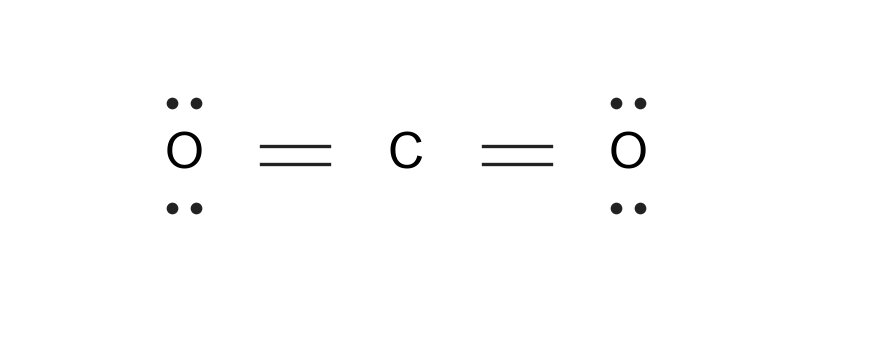
\includegraphics[width=0.86\linewidth]{rasmlar/gen/lw_864378.png}\end{center}
Molekulaning \textbf{formulasini aniqlang.}

\noindent A)~\textsl{Cl\textsubscript{2}} \hfill B)~\textsl{H\textsubscript{2}O} \hfill C)~\textsl{CO\textsubscript{2}} \hfill D)~\textsl{HCl}\par
\qsep
\noindent\qn{10.} Tabiiy elementning ikki izotopi: \textsuperscript{79}Br (50\%) va \textsuperscript{81}Br (50\%). Elementning o`rtacha nisbiy atom \textbf{massasini aniqlang.}

\noindent A)~\textsl{79} \hfill B)~\textsl{80} \hfill C)~\textsl{81} \hfill D)~\textsl{160}\par
\qsep
\noindent\qn{11.} Laboratoriyada Na\textsubscript{2}SO\textsubscript{4} eritmalari quyidagicha tayyorlangan:
\begin{center}
\renewcommand{\arraystretch}{1.15}
\fitbox{\begin{tabular}{|c|c|c|}\hline
\textbf{Idish} & \textbf{Eritma massasi, g} & \textbf{$\omega$(Na\textsubscript{2}SO\textsubscript{4}), \%} \\ \hline
A & 50 & 12 \\ \hline
B & 300 & 40 \\ \hline
\end{tabular}}
\end{center}
Bu ikki eritma bir idishga quyilib va ustiga 50 g suv qo`shilsa, yangi eritmadagi Na\textsubscript{2}SO\textsubscript{4} ning massa ulushi (\%) qancha bo`ladi?

\noindent A)~\textsl{26} \hfill B)~\textsl{52} \hfill C)~\textsl{31,5} \hfill D)~\textsl{16}\par
\qsep
\noindent\qn{12.} Jadvalda NaCl ning ikki eritmasi haqida ma'lumot berilgan:
\begin{center}
\renewcommand{\arraystretch}{1.15}
\fitbox{\begin{tabular}{|c|c|c|}\hline
\textbf{Eritma} & \textbf{Massasi, g} & \textbf{Massa ulushi, \%} \\ \hline
1 & 50 & 5 \\ \hline
2 & 300 & 30 \\ \hline
\end{tabular}}
\end{center}
Eritmalar aralashtirildi. Hosil bo`lgan eritmaning massa \textbf{ulushini (\%) aniqlang.}

\noindent A)~\textsl{17,5} \hfill B)~\textsl{26,43} \hfill C)~\textsl{35} \hfill D)~\textsl{8,57}\par
\qsep
\noindent\qn{13.} Faqat oksidlovchi bo`la oladigan \textbf{ionlarni aniqlang}: 1) Fe\textsuperscript{3+}; 2) S\textsuperscript{2$-$}; 3) Cl\textsuperscript{$-$}; 4) Zn\textsuperscript{2+}

\noindent A)~\textsl{3} \hfill B)~\textsl{4} \hfill C)~\textsl{3, 4} \hfill D)~\textsl{2}\par
\qsep
\noindent\qn{14.} D-metallar va ularning birikmalari haqida qaysi fikrlar to`g`ri? 1) Fe(OH)\textsubscript{2} havoda qo`ng`ir rangga o`tadi; 2) Xrom (VI) oksidi (CrO\textsubscript{3}) kislotali oksid; 3) Cu(OH)\textsubscript{2} qizdirilganda CuO ga parchalanadi; 4) Temir sovuq konsentrlangan HNO\textsubscript{3} da passivlanadi

\noindent\begin{tabular}{@{}p{0.47\linewidth}@{}p{0.47\linewidth}@{}}
A)~\textsl{2, 3, 4} & B)~\textsl{1, 2, 4} \\
C)~\textsl{1, 3, 4} & D)~\textsl{1, 2, 3, 4} \\
\end{tabular}\par
\qsep
\noindent\qn{15.} Reaksiya tenglamasi: Mg(HCO\textsubscript{3})\textsubscript{2} $\to$ MgCO\textsubscript{3} + CO\textsubscript{2} + H\textsubscript{2}O. Reaksiyaga tarkibida 20\% aralashma bo`lgan 36,5 g namuna (asosiy modda Mg(HCO\textsubscript{3})\textsubscript{2}) kirishdi. CO\textsubscript{2} \textbf{massasini (g) hisoblang.}

\noindent A)~\textsl{17,6} \hfill B)~\textsl{4,4} \hfill C)~\textsl{13,2} \hfill D)~\textsl{8,8}\par
\qsep
\noindent\qn{16.} SO\textsubscript{3} + 2KOH $\to$ K\textsubscript{2}SO\textsubscript{4} + H\textsubscript{2}O jarayoni uchun 80 g SO\textsubscript{3} olingan. KOH \textbf{massasini (g) aniqlang.}

\noindent A)~\textsl{28} \hfill B)~\textsl{224} \hfill C)~\textsl{112} \hfill D)~\textsl{56}\par
\qsep
\noindent\qn{17.} BaCl\textsubscript{2} + Na\textsubscript{2}SO\textsubscript{4} $\to$ BaSO\textsubscript{4} + 2NaCl reaksiyasida tarkibida 20\% aralashma bo`lgan 260 g namuna (asosiy modda BaCl\textsubscript{2}) ishtirok etdi. BaSO\textsubscript{4} \textbf{massasini (g) toping.}

\noindent A)~\textsl{233} \hfill B)~\textsl{466} \hfill C)~\textsl{116,5} \hfill D)~\textsl{349,5}\par
\qsep
\noindent\qn{18.} Quyidagi mineral o`g`itlardan qaysilari fosforli o`g`itlar jumlasiga kiradi? 1) Ca(H\textsubscript{2}PO\textsubscript{4})\textsubscript{2}; 2) Ca\textsubscript{3}(PO\textsubscript{4})\textsubscript{2}; 3) K\textsubscript{2}SO\textsubscript{4}; 4) (NH\textsubscript{4})\textsubscript{2}HPO\textsubscript{4}

\noindent A)~\textsl{3, 4} \hfill B)~\textsl{1, 2} \hfill C)~\textsl{1, 4} \hfill D)~\textsl{2, 3}\par
\qsep
\noindent\qn{19.} Reaksiya tenglamasi: 2NaNO\textsubscript{3} $\to$ 2NaNO\textsubscript{2} + O\textsubscript{2}. Reaksiyaga 17 g NaNO\textsubscript{3} kirishdi. NaNO\textsubscript{2} \textbf{massasini (g) hisoblang.}

\noindent A)~\textsl{27,6} \hfill B)~\textsl{6,9} \hfill C)~\textsl{20,7} \hfill D)~\textsl{13,8}\par
\qsep
\noindent\qn{20.} 15 g C\textsubscript{2}H\textsubscript{6} dan quyidagi ikki bosqichda C\textsubscript{2}H\textsubscript{5}OH olinadi: 1) C\textsubscript{2}H\textsubscript{6} + Cl\textsubscript{2} $\to$ C\textsubscript{2}H\textsubscript{5}Cl + HCl (unum 60\%); 2) C\textsubscript{2}H\textsubscript{5}Cl + KOH $\to$ C\textsubscript{2}H\textsubscript{5}OH + KCl (unum 75\%). Oxirgi mahsulot C\textsubscript{2}H\textsubscript{5}OH ning \textbf{massasini (g) toping.}

\noindent A)~\textsl{10,35} \hfill B)~\textsl{17,25} \hfill C)~\textsl{13,8} \hfill D)~\textsl{23}\par
\qsep
\noindent\qn{21.} Alken, alkadiyen va alkinlar haqida qaysi fikrlar to`g`ri? 1) Propenga HBr birikishi Markovnikov qoidasiga bo`ysunadi; 2) Alkinlar uchun umumiy formula CnH\textsubscript{2}n+2; 3) Alkenlar KMnO\textsubscript{4} ning suvli eritmasi bilan glikol hosil qiladi; 4) Asetilenni Kucherov reaksiyasi bilan sirka aldegidiga aylantirish mumkin

\noindent A)~\textsl{1, 3, 4} \hfill B)~\textsl{1, 2} \hfill C)~\textsl{2, 3, 4} \hfill D)~\textsl{3, 4}\par
\qsep
\noindent\qn{22.} Arenlar, neft va tabiiy gaz haqida qaysi fikrlar to`g`ri? 1) Naftalin -- bir halqali aren; 2) Benzol uchun birikish reaksiyalari mutlaqo xos emas; 3) Benzolda 6 ta sp\textsuperscript{2} gibridlangan uglerod bor; 4) Tabiiy gazning asosiy qismi propan

\noindent A)~\textsl{2, 3} \hfill B)~\textsl{3} \hfill C)~\textsl{1, 4} \hfill D)~\textsl{3, 4}\par
\qsep
\noindent\qn{23.} Reaksiya tenglamasi: C\textsubscript{6}H\textsubscript{5}OH + NaOH $\to$ C\textsubscript{6}H\textsubscript{5}ONa + H\textsubscript{2}O. Reaksiyaga tarkibida 75\% aralashma bo`lgan 32 g namuna (asosiy modda NaOH) kirishdi. C\textsubscript{6}H\textsubscript{5}OH \textbf{massasini (g) hisoblang.}

\noindent A)~\textsl{18,8} \hfill B)~\textsl{37,6} \hfill C)~\textsl{9,4} \hfill D)~\textsl{28,2}\par
\qsep
\noindent\qn{24.} Aldegid va ketonlar haqida qaysi fikrlar to`g`ri? 1) Aseton Cu(OH)\textsubscript{2} ni qaytaradi; 2) Formalin --- formaldegidning 40\% li eritmasi; 3) Formaldegid gaz holatda, suvda yaxshi eriydi; 4) Sirka aldegid Kucherov reaksiyasi bilan olinadi

\noindent A)~\textsl{2, 4} \hfill B)~\textsl{2, 3} \hfill C)~\textsl{2, 3, 4} \hfill D)~\textsl{1, 3}\par
\qsep
\noindent\qn{25.} C\textsubscript{4}H\textsubscript{10} alkanning izomerlari soni nechta?

\noindent A)~\textsl{2} \hfill B)~\textsl{3} \hfill C)~\textsl{1} \hfill D)~\textsl{4}\par
\qsep
\noindent\qn{26.} 442 g triolein (M = 884) nikel katalizatori ishtirokida to`liq gidrogenlandi. Sarflangan vodorod \textbf{hajmini (l, n.sh.) aniqlang.}

\noindent A)~\textsl{11,2} \hfill B)~\textsl{67,2} \hfill C)~\textsl{33,6} \hfill D)~\textsl{16,8}\par
\qsep
\noindent\qn{27.} Uglevodlar haqida qaysi fikrlar to`g`ri? 1) Maltoza gidrolizlanganda ikki molekula glyukoza hosil qiladi; 2) Kraxmal yod bilan ko`k rang beradi; 3) Selluloza $\beta$-glyukoza qoldiqlaridan iborat; 4) Fruktoza ketospirt

\noindent\begin{tabular}{@{}p{0.47\linewidth}@{}p{0.47\linewidth}@{}}
A)~\textsl{2, 3, 4} & B)~\textsl{1, 2, 3, 4} \\
C)~\textsl{1, 3, 4} & D)~\textsl{1, 2, 4} \\
\end{tabular}\par
\qsep
\noindent\qn{28.} Aminlar, aminokislotalar va oqsillar haqida qaysi fikrlar to`g`ri? 1) Dipeptidda 2 ta peptid bog` bor; 2) Anilin bromli suv bilan oq cho`kma beradi; 3) Oqsillar biuret reaksiyasini beradi; 4) Glitsin optik faol

\noindent A)~\textsl{4} \hfill B)~\textsl{1} \hfill C)~\textsl{2, 3} \hfill D)~\textsl{1, 2}\par
\qsep
\noindent\qn{29.} Reaksiya tenglamasi: C\textsubscript{2}H\textsubscript{4} + Cl\textsubscript{2} $\to$ C\textsubscript{2}H\textsubscript{4}Cl\textsubscript{2}. Reaksiyaga 7 g C\textsubscript{2}H\textsubscript{4} kirishdi. C\textsubscript{2}H\textsubscript{4}Cl\textsubscript{2} \textbf{massasini (g) hisoblang.}

\noindent A)~\textsl{49,5} \hfill B)~\textsl{24,75} \hfill C)~\textsl{12,38} \hfill D)~\textsl{37,12}\par
\qsep
\noindent\qn{30.} Rasmda ammiak olish tajribasi ko`rsatilgan. Qaysi moddalar aralashmasi qizdirilmoqda?
\begin{center}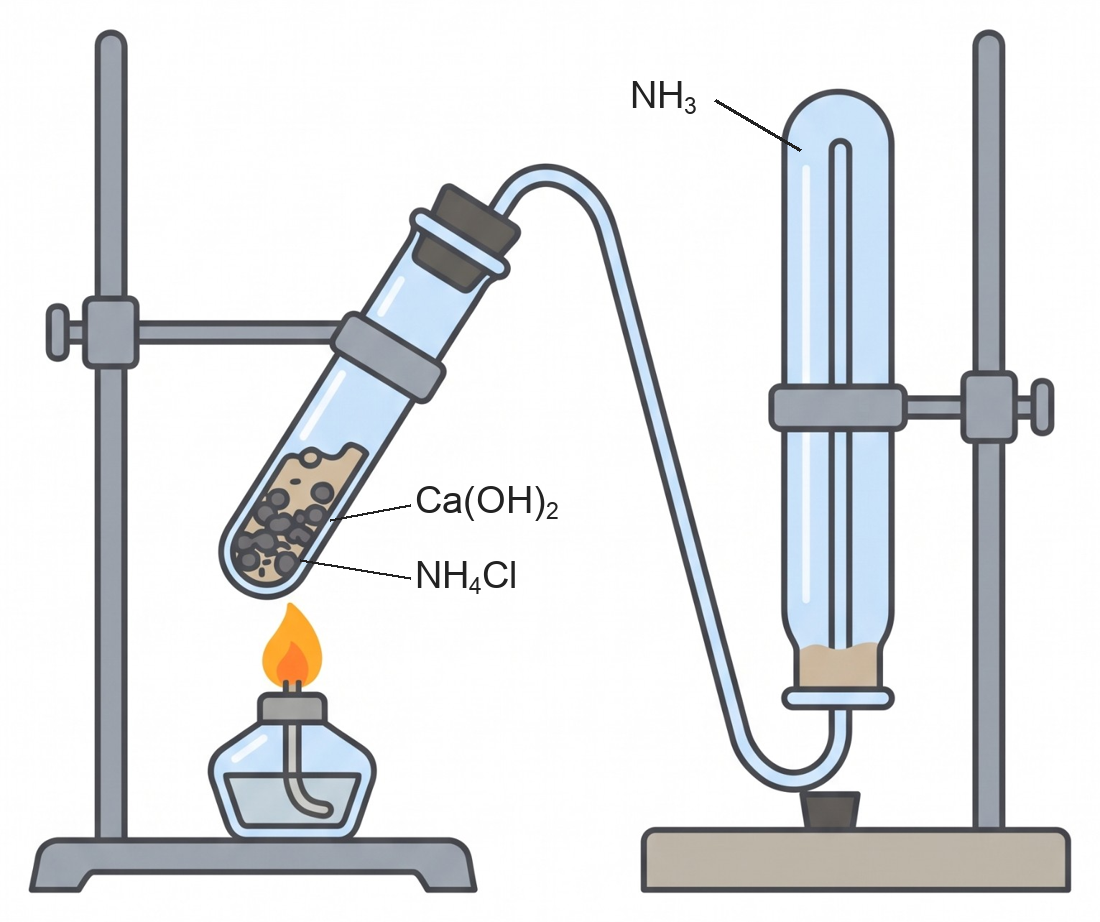
\includegraphics[width=0.86\linewidth]{rasmlar/darslik/d_nh3_lab.png}\end{center}

\noindent\begin{tabular}{@{}p{0.47\linewidth}@{}p{0.47\linewidth}@{}}
A)~\textsl{NH\textsubscript{4}Cl va Ca(OH)\textsubscript{2}} & B)~\textsl{NaCl va H\textsubscript{2}SO\textsubscript{4}} \\
C)~\textsl{Zn va HCl} & D)~\textsl{CaCO\textsubscript{3} va HCl} \\
\end{tabular}\par
\qsep
\noindent\qn{31.} 200 g 5\% li eritma tayyorlash uchun 50\% li eritmadan necha gramm olish kerak (qolgani suv)?

\noindent A)~\textsl{180} \hfill B)~\textsl{10} \hfill C)~\textsl{40} \hfill D)~\textsl{20}\par
\qsep
\noindent\qn{32.} Kimyoviy laboratoriyada pipetka nima uchun ishlatiladi?
\noindent A)~\textsl{qattiq moddalarni yuqori haroratda qizdirish}\par
\noindent B)~\textsl{titrlashda reagent hajmini aniq o`lchash}\par
\noindent C)~\textsl{vakuum ostida filtrlash}\par
\noindent D)~\textsl{eritmaning kichik hajmlarini o`lchab olish   ---}\par
\qsep
\end{multicols}
\medskip
\noindent\setlength{\fboxsep}{0pt}\fbox{\begin{tabular}{p{0.74\linewidth}|p{0.2\linewidth}}
\parbox[t]{0.72\linewidth}{\vspace{3pt}\textbf{Topshiriqlar (33--35) va javob variant (A--F)larini o`zaro to`g`ri moslashtiring.} Sirka kislota va etanoldan iborat 25,8 g aralashmaga mo`l NaHCO\textsubscript{3} eritmasi qo`shilganda 4,48 l (n.sh.) gaz ajraldi. Xuddi shunday massadagi aralashma natriy bilan ta'sirlashganda esa 5,6 l (n.sh.) vodorod ajraldi.
\vspace{3pt}} & \parbox[t]{0.19\linewidth}{\vspace{3pt}A~\textsl{6}\\[3pt]
B~\textsl{9,6}\\[3pt]
C~\textsl{12}\\[3pt]
D~\textsl{11,04}\\[3pt]
E~\textsl{13,12}\\[3pt]
F~\textsl{13,8}}\\ \hline
\parbox[t]{0.72\linewidth}{\vspace{2pt}\textbf{33. Aralashmadagi sirka kislota massasini (g) aniqlang.}\vspace{2pt}} & \\ \hline
\parbox[t]{0.72\linewidth}{\vspace{2pt}\textbf{34. Aralashmadagi etanol massasini (g) aniqlang.}\vspace{2pt}} & \\ \hline
\parbox[t]{0.72\linewidth}{\vspace{2pt}\textbf{35. Aralashma to`liq neytrallanganda (faqat kislota) hosil bo`lgan natriy atsetat massasini (g) aniqlang (reaksiya unumi 80\%).}\vspace{2pt}} & 
\end{tabular}}
\par\bigskip
\noindent\qn{36.} K\textsubscript{2}Cr\textsubscript{2}O\textsubscript{7} + KI + H\textsubscript{2}SO\textsubscript{4} $\to$ Cr\textsubscript{2}(SO\textsubscript{4})\textsubscript{3} + I\textsubscript{2} + K\textsubscript{2}SO\textsubscript{4} + H\textsubscript{2}O reaksiya tenglamasini tenglang. Oksidlovchi va qaytaruvchi oldidagi koeffitsiyentlar \textbf{yig`indisini aniqlang.}
\javob\qsep
\noindent\qn{37.} 14 g Fe reaksiyaga kirishdi (Fe + 2HCl $\to$ FeCl\textsubscript{2} + H\textsubscript{2}). Ajralgan H\textsubscript{2} \textbf{hajmini (l, n.sh.) hisoblang} (unum 90\%).
\javob\qsep
\noindent\qn{38.} 75,2 g Cu(NO\textsubscript{3})\textsubscript{2} qizdirilganda qisman parchalandi, qattiq qoldiq massasi 53,6 g bo`ldi. Ajralgan gazlar (n.sh.) \textbf{hajmini (l) hisoblang.}
\javob\qsep
\noindent\qn{39.} Etilen va asetilendan iborat 3,36 l (n.sh.) aralashma bromli suvdan o`tkazilganda 40 g brom yutildi. Aralashmadagi asetilenning \textbf{hajmini (l, n.sh.) toping.}
\javob\qsep
\noindent\qn{40.} 18 g sirka kislota va 6,4 g metanol dan 80\% unum bilan murakkab efir olindi. Efir \textbf{massasini (g) toping.}
\javob\qsep
\par\bigskip\begin{center}\textbf{\fontsize{13}{15}\selectfont YOZMA ISH}\end{center}
\noindent\qn{41.} \textbf{Topshiriqni bajarish jarayonida barcha reaksiya tenglamalarini yozing. Miqdoriy va arifmetik hisoblashlarni (unga asos bo`lgan usul yoki formulani ko`rsatgan holda) uzviy ketma-ketlikda bajaring.}\par\smallskip
Hajmi 1 l bo`lgan idishga 0,4 mol SO\textsubscript{2} va ma'lum miqdorda O\textsubscript{2} solindi hamda katalizator ishtirokida qizdirildi: 2SO\textsubscript{2} + O\textsubscript{2} $\rightleftarrows$ 2SO\textsubscript{3}. Muvozanat qaror topganda idishda SO\textsubscript{2}, O\textsubscript{2} va SO\textsubscript{3} ning mol nisbati 1 : 1 : 3 bo`ldi.\par
Hosil bo`lgan SO\textsubscript{3} ning hammasi 100 g 30\% li H\textsubscript{2}SO\textsubscript{4} eritmasiga yuttirildi (oleum hosil bo`lmadi, SO\textsubscript{3} to`liq suv bilan reaksiyaga kirishdi). Olingan eritmaga mo`l BaCl\textsubscript{2} eritmasi qo`shildi.\par
\noindent 1)\ O\textsubscript{2} ning boshlang`ich miqdorini (mol) va muvozanat konstantasini (K) hisoblang.\par
\noindent 2)\ SO\textsubscript{2} ning necha foizi reaksiyaga kirishgan? Muvozanatda SO\textsubscript{3} ning hajmiy ulushini (\%) ham toping.\par
\noindent 3)\ SO\textsubscript{3} yuttirilgandan keyingi eritmada H\textsubscript{2}SO\textsubscript{4} ning massa ulushini (\%) aniqlang.\par
\noindent 4)\ BaCl\textsubscript{2} qo`shilganda hosil bo`lgan cho`kma massasini (g) toping. BaCl\textsubscript{2} sarfini (g) ham toping.\par
\noindent 5)\ Doimiy haroratda idish hajmi 2 marta kamaytirilsa (v = k$\cdot$[SO\textsubscript{2}]\textsuperscript{2}$\cdot$[O\textsubscript{2}]), to`g`ri reaksiya tezligi necha marta o`zgaradi? Shuningdek muvozanatda umumiy bosimning boshlang`ich bosimga nisbatini (T = const) toping.\par
\diqqat{Mazkur topshiriq kengaytirilgan javobni talab etib, uning yechilish usuli va shu usul asosidagi barcha hisoblash amallari javoblar varaqasida aks etishi lozim.}\qsep
\noindent\qn{42.} Quyidagi o`zgarishlar zanjirida \textit{X}, \textit{Y}, \textit{Z} noma'lum organik moddalar:\par
\[\setlength{\fboxsep}{0pt}\text{C\textsubscript{2}H\textsubscript{5}Cl}\xrightarrow{\text{KOH (spirtli)}}\text{\textit{X}}\xrightarrow{\text{Br\textsubscript{2}}}\text{\textit{Y}}\xrightarrow{\text{KOH (spirtli)}}\text{\textit{Z}}\xrightarrow{\text{C (aktiv), 600 \textdegree{}C}}\text{C\textsubscript{6}H\textsubscript{6}}\]
\noindent 1)\ C\textsubscript{2}H\textsubscript{5}Cl $\to$ \textit{X} : reaksiya tenglamasini yozing; hosil bo`lgan moddani nomlang.\par
\noindent 2)\ \textit{X} $\to$ \textit{Y} : reaksiya tenglamasini yozing; hosil bo`lgan moddani nomlang.\par
\noindent 3)\ \textit{Y} $\to$ \textit{Z} : reaksiya tenglamasini yozing; hosil bo`lgan moddani nomlang.\par
\noindent 4)\ \textit{Z} $\to$ C\textsubscript{6}H\textsubscript{6} : reaksiya tenglamasini yozing; hosil bo`lgan moddani nomlang.\par
\diqqat{Mazkur topshiriq kengaytirilgan javobni talab etib, uning yechilish usuli va shu usul asosidagi barcha hisoblash amallari javoblar varaqasida aks etishi lozim.}\qsep
\noindent\qn{43.} \textbf{Topshiriqni bajarish jarayonida barcha reaksiya tenglamalarini yozing. Miqdoriy va arifmetik hisoblashlarni (unga asos bo`lgan usul yoki formulani ko`rsatgan holda) uzviy ketma-ketlikda bajaring.}\par\smallskip
67,2 l (n.sh.) ammiak katalizator ishtirokida kislorodda oksidlandi (4NH\textsubscript{3} + 5O\textsubscript{2} $\to$ 4NO + 6H\textsubscript{2}O, unum 80\%). Hosil bo`lgan NO ni nitrat kislotagacha qayta ishlash unumi 80\%.\par
\noindent 1)\ Hosil bo`lgan NO hajmini (l, n.sh.) hisoblang. Hosil bo`lgan NO ning massasini (g) ham toping.\par
\noindent 2)\ Nitrat kislota ishlab chiqarishning keyingi bosqichlari tenglamalarini yozing va olingan HNO\textsubscript{3} massasini (g) toping.\par
\noindent 3)\ Hosil bo`lgan HNO\textsubscript{3} ni to`liq neytrallash uchun zarur ammiak hajmini (l, n.sh.) aniqlang (NH\textsubscript{3} + HNO\textsubscript{3} $\to$ NH\textsubscript{4}NO\textsubscript{3}).\par
\noindent 4)\ Hosil bo`lgan ammoniy nitrat massasini (g) hisoblang va azotning massa ulushini (\%) toping.\par
\noindent 5)\ Olingan HNO\textsubscript{3} dan 63\% li eritma necha gramm tayyorlanadi?\par
\diqqat{Mazkur topshiriq kengaytirilgan javobni talab etib, uning yechilish usuli va shu usul asosidagi barcha hisoblash amallari javoblar varaqasida aks etishi lozim.}\qsep
\newpage
\noindent\textbf{\fontsize{13}{15}\selectfont 15-variant}\hfill \textbf{Javoblar kaliti}\par\smallskip\hrule\smallskip
\textit{Faqat o`qituvchi uchun.}\par\medskip
\noindent\textbf{1--32-savollar}\par\smallskip
\noindent\begin{tabular}{|c|c|c|c|c|c|c|c|c|c|c|c|c|c|c|c|}\hline
\textbf{1} & \textbf{2} & \textbf{3} & \textbf{4} & \textbf{5} & \textbf{6} & \textbf{7} & \textbf{8} & \textbf{9} & \textbf{10} & \textbf{11} & \textbf{12} & \textbf{13} & \textbf{14} & \textbf{15} & \textbf{16}\\\hline
\textsl{C} & \textsl{A} & \textsl{D} & \textsl{B} & \textsl{A} & \textsl{D} & \textsl{D} & \textsl{C} & \textsl{C} & \textsl{B} & \textsl{C} & \textsl{B} & \textsl{B} & \textsl{D} & \textsl{D} & \textsl{C}\\\hline
\textbf{17} & \textbf{18} & \textbf{19} & \textbf{20} & \textbf{21} & \textbf{22} & \textbf{23} & \textbf{24} & \textbf{25} & \textbf{26} & \textbf{27} & \textbf{28} & \textbf{29} & \textbf{30} & \textbf{31} & \textbf{32}\\\hline
\textsl{A} & \textsl{B} & \textsl{D} & \textsl{A} & \textsl{A} & \textsl{B} & \textsl{A} & \textsl{C} & \textsl{A} & \textsl{C} & \textsl{B} & \textsl{C} & \textsl{B} & \textsl{A} & \textsl{D} & \textsl{D}\\\hline
\end{tabular}\par\medskip
\noindent\textbf{33--35-savollar}\par\smallskip
\noindent\begin{tabular}{|c|c|c|}\hline \textbf{No} & \textbf{Javob} & \textbf{Qiymat}\\\hline
33 & \textsl{C} & 12\\\hline
34 & \textsl{F} & 13,8\\\hline
35 & \textsl{E} & 13,12\\\hline
\end{tabular}\par\medskip
\noindent\textbf{36--40-savollar}\par\smallskip
\noindent\begin{tabular}{|c|c|}\hline \textbf{No} & \textbf{To`g`ri javob}\\\hline
36 & 7\\\hline
37 & 5,04\\\hline
38 & 11,2\\\hline
39 & 2,24\\\hline
40 & 11,84\\\hline
\end{tabular}\par\medskip
\noindent\textbf{41--43-topshiriqlar: javoblar}\par\smallskip
\noindent\textbf{41-topshiriq.}\par
\noindent 1) 0,25 mol; 90\par
\noindent 2) 75\%; 60\%\par
\noindent 3) 47,9\%\par
\noindent 4) 141,23 g; 126,07 g\par
\noindent 5) 8 marta ortadi; 0,77\par
\noindent\textbf{42-topshiriq.}\par
\noindent 1) C\textsubscript{2}H\textsubscript{5}Cl + KOH (spirtli) $\to$ C\textsubscript{2}H\textsubscript{4} (etilen)\par
\noindent 2) C\textsubscript{2}H\textsubscript{4} + Br\textsubscript{2} $\to$ C\textsubscript{2}H\textsubscript{4}Br\textsubscript{2} (1,2-dibrometan)\par
\noindent 3) C\textsubscript{2}H\textsubscript{4}Br\textsubscript{2} + KOH (spirtli) $\to$ C\textsubscript{2}H\textsubscript{2} (asetilen)\par
\noindent 4) C\textsubscript{2}H\textsubscript{2} + C (aktiv), 600 \textdegree{}C $\to$ C\textsubscript{6}H\textsubscript{6} (benzol)\par
\noindent\textbf{43-topshiriq.}\par
\noindent 1) 53,76 l; 72 g\par
\noindent 2) 120,96 g\par
\noindent 3) 43,01 l\par
\noindent 4) 153,6 g; 35\%\par
\noindent 5) 192 g\par
\par\bigskip\noindent\textbf{Mavzular taqsimoti}\par\smallskip
{\small\noindent\begin{longtable}{|c|p{7.2cm}|p{5.4cm}|c|}\hline \textbf{No} & \textbf{Mavzu} & \textbf{Tekshiriladigan ko`nikma} & \textbf{Ball}\\\hline
1 & Tirkashev I bob (kvant sonlari) & Bilim va tushunish & 1\\\hline
2 & 11-sinf (Faradey qonuni, grafik) & Grafik tahlili & 1\\\hline
3 & 11-sinf 4-bob (normal konsentratsiya) & Hisoblash va masala yechish & 1\\\hline
4 & 8-sinf (kimyoviy bog`lanish turlari, jadval) & Jadval tahlili & 1\\\hline
5 & 11-sinf 4-bob (normal konsentratsiya) & Hisoblash va masala yechish & 1\\\hline
6 & Tashev; 9-sinf (metallarning kuchlanish qatori) & Hisoblash va masala yechish & 1\\\hline
7 & 11-sinf (Mendeleyev--Klapeyron) & Hisoblash va masala yechish & 1\\\hline
8 & Tirkashev IV bob (kuchli elektrolitlar) & Hisoblash va masala yechish & 1\\\hline
9 & 8-sinf (kovalent bog`) & Rasm bo`yicha tahlil & 1\\\hline
10 & 8-sinf (izotoplar) & Hisoblash va masala yechish & 1\\\hline
11 & Tirkashev III bob (eritmalar, jadval) & Jadval tahlili & 1\\\hline
12 & Tirkashev III bob (eritmalar, jadval) & Jadval tahlili & 1\\\hline
13 & Tirkashev \textit{V} bob; 11-sinf 7-bob & Bilim va tushunish & 1\\\hline
14 & 9-sinf; Tashev (Fe, Cu, Zn, Cr) & Bilim va tushunish & 1\\\hline
15 & 9-sinf; Tirkashev (suv qattiqligi, hisob) & Hisoblash va masala yechish & 1\\\hline
16 & 9-sinf; Tirkashev (oksid/asos/kislota/tuz, hisob) & Hisoblash va masala yechish & 1\\\hline
17 & 9-sinf; Tirkashev (genetik zanjir/reaksiya turlari, hisob) & Hisoblash va masala yechish & 1\\\hline
18 & Tashev (mineral o`g`itlar) & Bilim va tushunish & 1\\\hline
19 & 9-sinf; Tirkashev (tuzlarning termik parchalanishi, hisob) & Hisoblash va masala yechish & 1\\\hline
20 & 10-sinf (ikki bosqichli hisob) & Hisoblash va masala yechish & 1\\\hline
21 & 10-sinf (mavzuga oid paragraflar); Abdusamatov & Bilim va tushunish & 1\\\hline
22 & 10-sinf (mavzuga oid paragraflar); Abdusamatov & Bilim va tushunish & 1\\\hline
23 & 10-sinf (spirt, hisob) & Hisoblash va masala yechish & 1\\\hline
24 & 10-sinf (mavzuga oid paragraflar); Abdusamatov & Bilim va tushunish & 1\\\hline
25 & 10-sinf \S{}6, \S{}12, \S{}20, \S{}28 (izomeriya) & Bilim va tushunish & 1\\\hline
26 & 10-sinf \S{}29 (yog`larni gidrogenlash) & Hisoblash va masala yechish & 1\\\hline
27 & 10-sinf (mavzuga oid paragraflar); Abdusamatov & Bilim va tushunish & 1\\\hline
28 & 10-sinf (mavzuga oid paragraflar); Abdusamatov & Bilim va tushunish & 1\\\hline
29 & 10-sinf (pol, hisob) & Hisoblash va masala yechish & 1\\\hline
30 & 8-sinf (23-rasm) & Rasm bo`yicha tahlil & 1\\\hline
31 & Tirkashev III bob (eritma tayyorlash) & Hisoblash va masala yechish & 1\\\hline
32 & 7-sinf (laboratoriya jihozlari) & Bilim va tushunish & 1\\\hline
33--35 & Aralash masala (moslashtirish) & Ko`p bosqichli hisob & 3\\\hline
36--40 & Qisqa javobli masalalar & Hisoblash & 5\\\hline
41--43 & Yozma ish & Usul va hisob (M, A) & 75\\\hline
\end{longtable}}
\end{document}
